\chapter{Implementasi dan Pengujian}

Bab ini akan membahas seluruh proses implementasi yang dilakukan untuk menerapkan rancangan yang sudah didefinisikan sebelumnya. Selain itu, bab ini juga akan membahas pengujian yang dilakukan terhadap hasil implementasi yang mencakup hal-hal yang diuji, metode pengujian, dan hasil pengujian yang diperoleh. 


\section{Implementasi}
Implementasi sistem \textit{Performance Regression Analysis} (PRA) akan dibuat berdasarkan rancangan arsitektur seperti yang terdapat pada gambar \ref{arch-pra}. Komponen seperti \textit{library} instrumentasi, melainkan akan melakukan \textit{fork} dan modifikasi solusi \textit{Open Source} \textit{distributed tracing} dari Zipkin. Komponen yang akan dibuat dari awal sepenuhnya adalah \textit{User Interface} (UI) dan \textit{engine} dari sistem PRA yang akan melakukan komputasi utama sistem pendeteksian dan analisis regresi. Komponen \textit{engine} juga akan berfungsi sebagai API yang akan diakses oleh komponen \textit{User Interface}.



\subsection{Implementasi \textit{Performance Regression Analysis} \textit{engine}}

Sebelum melakukan implementasi solusi, penulis harus terlebih dahulu melakukan pemilihan kakas yang akan digunakan melakukan implementasinya. Secara umum, terdapat banyak bahasa pemrograman yang dapat melakukan implementasi solusi komponeasdn \textit{engine} sesuai dengan alur yang terdapat pada gambar \ref{alur-pra}. Namun, ada suatu kebutuhan penting untuk melakukan tes statistik Kolmogorov-Smirnov (K-S) yang tidak semua bahasa pemrograman memiliki dukungan \textit{library} untuk melakukannya. Terdapat dua bahasa pemrograman yang memiliki \textit{library} untuk melakukan tes K-S yaitu bahasa pemrograman \textbf{Go} dan \textbf{Python}. Bahasa \textbf{Go} memiliki library Gonum \footnote{\url{gonum.org}} yang memiliki implementasi tes K-S dalam fungsi \texttt{KolmogorovSmirnov}, sementara bahasa \textbf{Python} memiliki library SciPy \footnote{\url{scipy.org}} yang memiliki implementasi tes K-S dalam fungsi \texttt{scipy.stat.ks\textunderscore 2samp}.

Dari kedua bahasa tersebut, penulis memilih bahasa \textbf{Python} untuk melakukan implementasi solusi setelah berhasil melakukan \textit{parsing} data \textit{trace} Zipkin dengan pendekatan pemrograman berorientasi objek yang didasarkan pada \textit{source code} yang dimiliki oleh aplikasi \textit{User Interface} milik Zipkin yang diimplementasikan dengan bahasa \textbf{Javascript}. 

Implementasi \textit{engine} akan terbagi menjadi beberapa modul seperti yang terlihat pada tabel \ref{engine-module}.

\begin{small}
	\begin{longtable}{ | p{1cm} | p{3cm} | p{10cm} | }
		\caption{Tabel pembagian modul komponen \textit{engine}}
		\label{engine-module}                                                           
		\\ \hline
		\centering\bfseries{ID} & \centering\bfseries{Nama Modul} & \centering\bfseries{Deskripsi} \tabularnewline \hline
		\endfirsthead
		EM-1 & zipkin (Pengambilan Data) & Modul ini bertanggung jawab untuk mengambil data dari API Zipkin yang memiliki data hasil \textit{trace} dari aplikasi. \\ \hline
		EM-2 & transform (Transformasi Data) & Modul ini bertanggung jawab untuk melakukan transformasi dari data \textit{trace} mentah yang diambil dari API Zipkin menjadi bentuk-bentuk model yang akan digunakan untuk komputasi di tahap selanjutnya seperti sampel data \textit{latency}, dan model data \textit{Critical Path}. Semua model akan disimpan dalam data berbentuk JSON. \\ \hline
		EM-3 & storage (Penyimpanan Data) & Modul ini bertanggung jawab untuk menyimpan model hasil transformasi \textit{baseline} dari modul EM-2 ke \textit{storage} untuk digunakan kembali pada fase \textit{Real-time Analysis}. Komponen \textit{storage} yang akan digunakan adalah Redis. Alasan utama pemilihan Redis sebagai komponen \textit{storage} adalah Redis telah memiliki modul penyimpanan data dalam bentuk JSON dan memiliki kinerja yang tinggi sebab data disimpan secara \textit{in-memory}. \\ \hline
		EM-4 & statistic (Perhitungan Statistik) & Modul ini bertanggung jawab untuk melakukan komputasi perhitungan statistik yang mencakup pendeteksian regresi dengan menghitung koefisien Kolmogorov-Smirnov seperti yang telah dijelaskan pada subbab \ref{approach-cumulative} menggunakan fungsi yang disediakan oleh library SciPy. \\ \hline
		EM-5 & critical\textunderscore path (Analisis \textit{Critical Path}) & Modul ini bertanggung jawab untuk melakukan analisis \textit{Critical Path} yang bertujuan untuk mencari penyebab regresi dengan mencari \textit{Critical Path} dari tiap \textit{service} dan melihat perbandingan \textit{latency} dari operasi tersebut dengan \textit{latency} yang telah direkam sebelumnya pada fase \textit{Baseline Loading}. Operasi yang selisih \textit{latency}-nya melebihi \textit{threshold} diduga kuat merupakan penyebab utama dari regresi yang terjadi. \\ \hline
		EM-6 & scheduling (\textit{Scheduling}) & Pada modul ini akan diimplentasikan \textit{job} atau pekerjaan utama yang akan digunakan untuk melakukan analisis regresi dengan menggunakan fungsi-fungsi yang telah diimplementasikan pada modul-modul sebelumnya dan juga bertanggung jawab melakukan penjadwalan \textit{job} tertentu selama interval yang ditentukan.  \\ \hline
	\end{longtable}
\end{small}

Aplikasi \textit{engine} akan dibuat sebagai REST API dan akan diimplementasikan menggunakan \textit{framework} FastAPI. Fungsionalitas \textit{engine} akan diekspos melalui REST API sehingga dapat digunakan baik oleh komponen UI maupun langsung melalui pemanggilan HTTP untuk keperluan pengujian. Beberapa \textit{endpoint} yang akan diimplementasikan terlihat pada tabel \ref{endpoints}.

\begin{small}
	\begin{longtable}{ | p{1cm} | p{2cm} | p{3.5cm} | p{7.5cm} | }
		\caption{Tabel \textit{endpoint} API \textit{engine}}
		\label{endpoints}                                                           
		\\ \hline
		\centering\bfseries{ID} & \centering\bfseries{Operasi HTTP} & \centering\bfseries{\textit{endpoint}} & \centering\bfseries{Deskripsi} \tabularnewline \hline
		\endfirsthead
		EP-1 & \centering{GET} & \centering\texttt{/state} & Data \textit{state} dari \textit{engine} yang akan berisikan informasi mengenai status pendeteksian regresi, pengecekan terakhir regresi, dan hasil analysis \textit{critical path} yang diduga menjadi penyebab regresi. \\ \hline
		EP-2 & \centering{POST} & \centering\texttt{/baseline} & Dengan \textit{endpoint} ini, \textit{user} dapat membuat \textit{engine} mengambil data \textit{baseline} baru dengan menyuplai informasi mengenai waktu mulai dan waktu selesai \textit{trace} di Zipkin beserta dengan batas banyaknya \textit{trace} yang akan diambil. \\ \hline
		EP-3 & \centering{DELETE} & \centering\texttt{/baseline} & \textit{Endpoint} ini akan menghapus informasi mengenai \textit{baseline} yang ada di data \textit{state}. \\ \hline	
		EP-4 & \centering{GET} & \centering\texttt{/analysis/range} & \textit{Endpoint} ini berfungsi untuk memicu \textit{engine} untuk melakukan analisis regresi dengan informasi waktu mulai dan waktu selesai trace yang disuplai oleh pengguna melalui \textit{query parameter}. API kemudian akan mengembalikan hasil analisis berupa apakah regresi terdeteksi beserta analisis \textit{critical path}. \\ \hline
		EP-5 & \centering{GET} & \centering\texttt{/analysis/realtime} & \textit{Endpoint} ini berfungsi untuk memicu \textit{engine} untuk melakukan analisis regresi dengan informasi waktu mulai dan waktu selesai trace yang telah ditentukan sebelumnya dan juga melakukan \textit{update} informasi state dengan hasil analisis regresi yang telah dilakukan. API kemudian akan mengembalikan hasil analisis berupa apakah regresi terdeteksi beserta analisis \textit{critical path}. \\ \hline				
	\end{longtable}
\end{small}

Secara umum, alur kerja endpoint EP-4 dan EP-5 serupa dengan perbedaan kecil waktu pengambilan \textit{trace} yang mana EP-4 dapat mengambil data \textit{trace} secara semaunya secara presisi sehingga endpoint ini akan digunakan untuk melakukan pengujian secara manual, sementara EP-5 digunakan untuk menyimulasikan tingkah laku dari \textit{engine} yang melakukan analisis dalam interval waktu tertentu tanpa harus menunggu interval waktunya.

Alur kerja analisis regresi pertama dimulai dengan mengambil data \textit{trace} yang akan dilakukan oleh module EM-1. Data \textit{trace} akan diambil dari API Zipkin dalam bentuk JSON dan akan dilakukan \textit{parsing} sehingga data akhir yang didapatkan mengandung informasi \textit{latency} dari semua \textit{span} yang terdaoat pada \textit{trace} tersebut. Setelah data \textit{trace} diambil dari API dan di-\textit{parse} oleh modul EM-1, selanjutnya data \textit{trace} tersebut akan ditransformasikan untuk diambil informasi \textit{latency}-nya oleh modul EM-2. Selanjutnya, dengan asumsi bahwa data \textit{baseline} telah didapatkan, \textit{engine} selanjutnya akan mengambil data \textit{latency} baseline yang akan dilakukan oleh modul EM-3. Setelah informasi \textit{latency} \textit{baseline} maupun \textit{realtime} sudah didapatkan, selanjutnya analisis pertama-tama dilakukan dengan menguji terjadinya regresi dengan fungsi statistik dari modul EM-4. Hasilnya adalah sebuah variabel \textit{boolean} yang melakukan tes K-S untuk menentukan apakah kedua sampel data tersebut berasal dari distribusi yang berbeda. Jika hasil tes menghasilkan kedua data berasal dari distribusi yang berbeda, dapat menjadi indikasi bahwa regresi telah terjadi. 

Jika terindikasi regresi telah terjadi, \textit{engine} selanjutnya akan melakukan analisis \textit{critical path}. Pertama-tama data \textit{trace} \textit{baseline} maupun \textit{realtime} akan ditransformasikan menjadi model \textit{critical path} oleh modul EM-2. Kemudian kedua model \textit{critical path} tersebut akan dibandingkan oleh modul EM-5 dan hasil akhirnya adalah data perbandingan operasi-operasi yang ada di data \textit{baseline} dan \textit{realtime}. Hasil akhir data pengecekan regresi dan analisis \textit{critical path} akan dikirim sebagai \textit{response} dalam bentuk JSON oleh API. Semua operasi dari alur kerja yang telah disebutkan di atas diimplementasikan dalam fungsi yang terdapat pada modul EM-6.

\subsubsection{Model dan Struktur Data}
Sistem PRA yang dibuat bergantung pada data \textit{trace} yang diperoleh dari Zipkin. Data tersebut tidak bisa begitu saja digunakan untuk menjalankan fungsi-fungsi dari \textit{engine} PRA sesuai yang terdapat pada gambar \ref{alur-pra} dan perlu ditransformasikan menjadi model dan struktur data yang lebih bermakna seperti yang telah disebutkan pada EM-2 di tabel \ref{engine-module}.

Dalam dokumentasinya, Zipkin menyediakan keterangan mengenai model data \textit{trace} yang digunakannya seperti yang terdapat pada \citep{zipkin-data}. Model data yang digunakan Zipkin terbagi menjadi dua yaitu \textit{span} dan \textit{trace}. \textit{Trace} sendiri merupakan serangkaian \textit{span} dengan id \textit{trace} sama yang merepresentasikan alur jalannya sebuah \textit{request} dalam sebuah \textit{service} yang telah terinstrumentasi, sementara \textit{span} merepresentasikan salah satu operasi yang terjadi sepanjang sebuah \textit{request}. Beberapa informasi yang terdapat pada data \textit{span} antara lain adalah informasi mengenai \textit{trace} dimana \textit{span} itu berada, metadata mengenai operasi yang direpresentasikan \textit{span}, durasi atau \textit{latency} dari operasi.

Sementara itu, untuk memenuhi fungsi-fungsi pada sistem PRA, data yang bersumber dari Zipkin perlu ditransformasikan menjadi struktur data yang sesuai dengan kebutuhan masing-masing tahap analisis. Dari rancangan alur sistem PRA, terdapat tiga tahap analisis yang akan dilakukan, yaitu tahap pendeteksian regresi dengan analisis statistik Kolmogorov-Smirnov, tahap analisis korelasi, dan tahap analisis \textit{critical path}.

Pada tahap pendeteksian regresi dengan tes statistik Kolmogorov-Smirnov (K-S), data yang diperlukan adalah data \textit{latency} atau durasi operasi dari \textit{span} yang dimiliki oleh Zipkin. Tes K-S akan membandingkan dua buah sampel data \textit{latency} dan akan menghasilkan hipotesis apakah kedua fungsi tersebut berada pada distribusi yang sama.

Pada tahap analisis \textit{critical path}, data yang dibutuhkan adalah pasangan \textit{key-value} dari nama operasi yang terrekam oleh Zipkin dan juga nilai \textit{latency} dari operasi tersebut. Data \textit{critical path} akan disimpan sebagai struktur data \textit{map} yang sesuai untuk menyimpan data berbentuk pasangan \textit{key-value}. Data ini akan didapatkan dari data \textit{trace} bawaan Zipkin yang sudah memiliki informasi mengenai \textit{critical path} dan juga nilai \textit{latency} nya masing-masing. 

\subsubsection{Algoritme penting}
Setelah pada subbab sebelumnya didefinisikan struktur data yang akan digunakan untuk merepresentasikan beberapa model seperti yang ada pada gambar \ref{alur-pra}, pada subbab ini akan didefinisikan beberapa algoritme penting dalam bentuk \textit{pseudocode} yang akan digunakan untuk melakukan berbagai operasi pada sistem PRA.

\begin{algorithm}[hbt!]
	\SetAlgorithmName{Algoritme}{Algoritme}
	
	\SetKwData{Left}{left}\SetKwData{This}{this}\SetKwData{Up}{up}
	\SetKwFunction{Union}{Union}\SetKwFunction{IsRegression}{IsRegression}
	\SetKwInOut{Input}{input}\SetKwInOut{Output}{output}
	\Input{Two array of float numbers representing latency: data1 and data2}
	\Output{Boolean indicating if regression has occured}
	\BlankLine
	
	
	\caption{Algoritme pendeteksian regresi}\label{alg:regression-detection}
\end{algorithm}
\begin{algorithm}[hbt!]
	\SetAlgorithmName{Algoritme}{Algoritme}
	
	
	
	
	\caption{Algoritme analisis regresi}\label{alg:regression-analysis}
\end{algorithm}

%\subsubsection{\textit{Deployment}}
%Agar aplikasi \textit{engine} dapat dijalankan di lingkungan Kubernetes, aplikasi harus dikemas dalam bentuk \textit{container} dan di-\textit{deploy} di Kubernetes menggunakan file \textit{manifest} berbentuk yaml. 

\subsubsection{Hasil implementasi}
Modul-modul pada tabel \ref{engine-module} masing-masing akan diimplementasikan sebagai \textit{package} pada bahasa \textit{Python} seperti yang terlihat pada gambar \ref{package}. Terdapat tujuh buah \textit{package}, enam buah \textit{package} dari modul dan satu buah \textit{package} \texttt{utils} yang berisi fungsi-fungsi untuk mendukung kerja fungsi di modul lainnya. Semua \textit{source code} hasil implementasi disimpan di Github \footnote{\url{https://github.com/masterraf21/pra\textunderscore engine}}.
\begin{figure}[!htb]
	\centering
	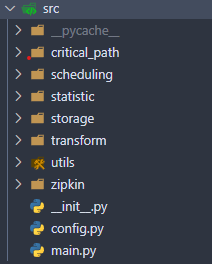
\includegraphics[width=0.4\textwidth]{resources/ch4/packages.png}
	\caption{Implementasi modul sebagai \textit{package}}
	\label{package}
\end{figure} 

Gambar \ref{api_docs} adalah hasil tangkapan layar dokumentasi API yang disediakan oleh FastAPI. 
\begin{figure}[!htb]
	\centering
	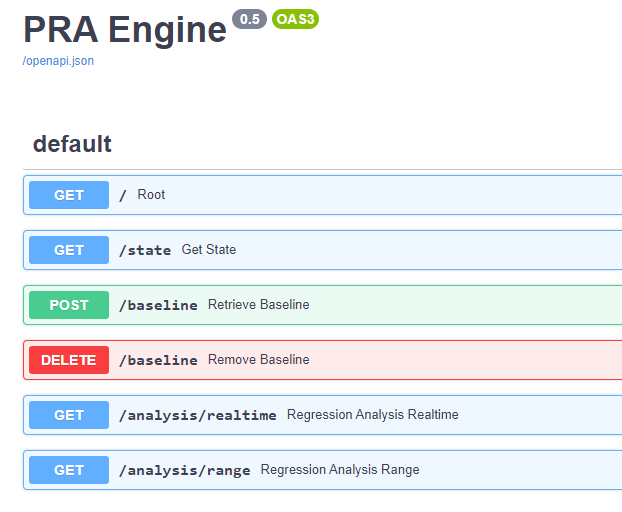
\includegraphics[width=0.6\textwidth]{resources/ch4/api_docs.png}
	\caption{Dokumentasi API}
	\label{api_docs}
\end{figure} 

Berikut adalah tangkapan layar dari hasil pemanggilan beberapa \textit{endpoint} yang dilakukan dengan aplikasi Postman \footnote{\url{https://www.postman.com/}}.
\begin{figure}[!ht]
	\centering
	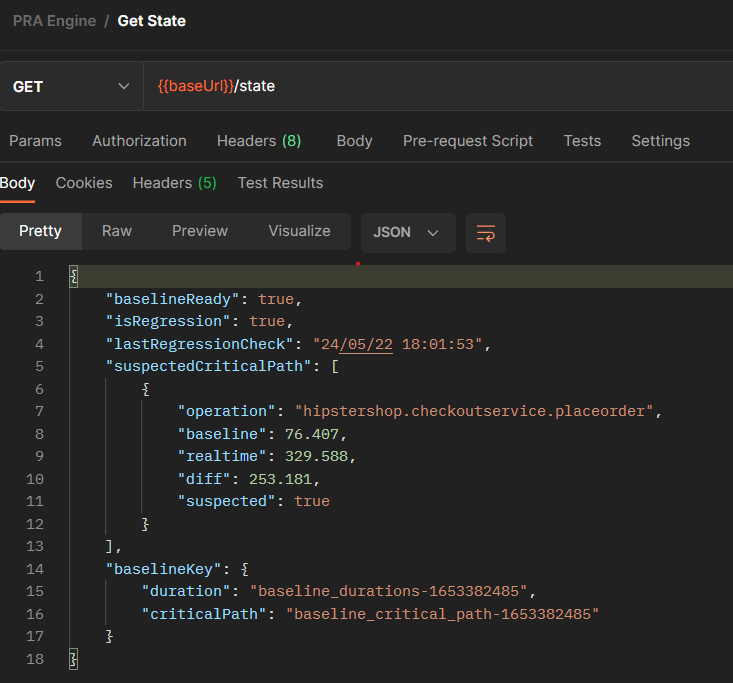
\includegraphics[width=0.75\textwidth]{resources/ch4/result_state.png}
	\caption{Hasil pemanggilan \textit{endpoint} \texttt{/state}}
	\label{api_state}
\end{figure} 
\begin{figure}[!ht]
	\centering
	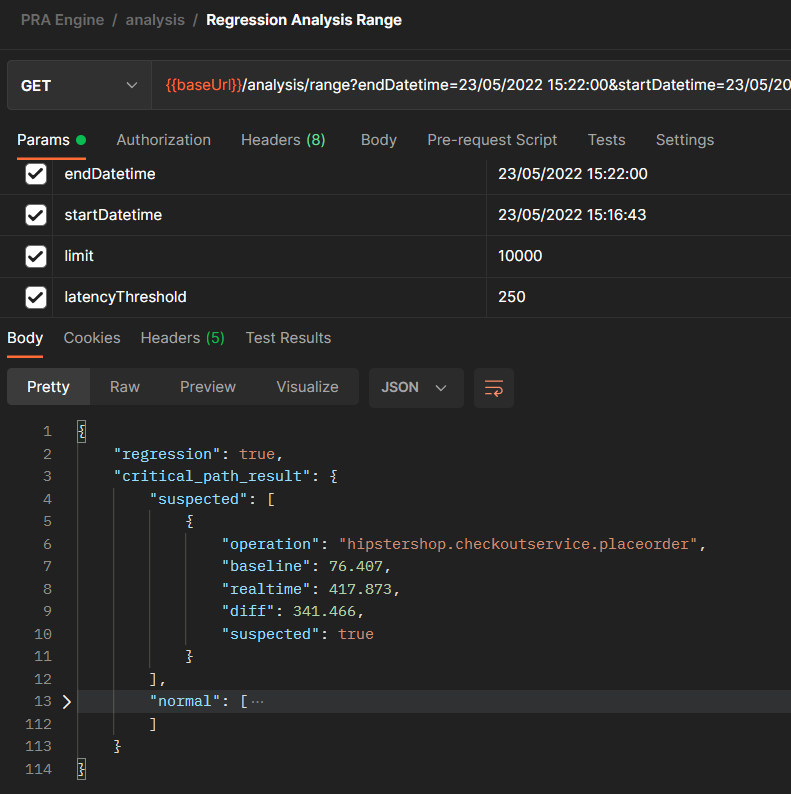
\includegraphics[width=0.75\textwidth]{resources/ch4/result_analysis_range.png}
	\caption{Hasil pemanggilan \textit{endpoint} \texttt{/analysis/range}}
	\label{api_analysis_range}
\end{figure} 
\begin{figure}[!ht]
	\centering
	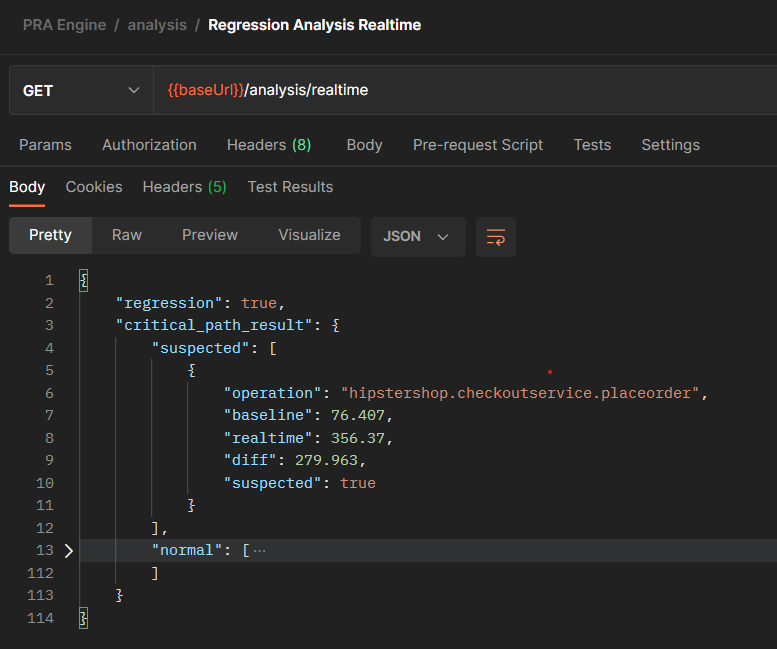
\includegraphics[width=0.75\textwidth]{resources/ch4/result_analysis_realtime.png}
	\caption{Hasil pemanggilan \textit{endpoint} \texttt{/analysis/realtime}}
	\label{api_analysis_realtime}
\end{figure} \\


\subsection{\textit{User Interface}}
Komponen lainnya yang akan diimplementasikan pada Tugas Akhir ini adalah komponen \textit{User Interface} (UI). Komponen ini akan menjadi antarmuka yang dapat digunakan untuk mengetahui \textit{state} dari sistem PRA. Fungsionalitas yang akan dibuat pada komponen UI akan dijabarkan pada tabel kebutuhan  fungsional \ref{ui-functional}.
\begin{small}
	\begin{longtable}{ | p{3cm} | p{9cm} | }
		\caption{Tabel kebutuhan fungsional komponen UI}
		\label{ui-functional}                                                           
		\\ \hline
		\centering\bfseries{ID} & \centering\bfseries{Deskripsi} \tabularnewline \hline
		\endfirsthead
		\centering{UI-1} & UI dapat menampilkan status pendeteksian regresi  \\ \hline
		\centering{UI-2} & UI dapat menampilkan hasil analisis \textit{critical path} berupa nama operasi dan nilai \textit{latency} \\ \hline

	\end{longtable}
\end{small}

\subsubsection{Hasil implementasi}
Berikut adalah tangkapan layar hasil implementasi komponen \textit{User Interface}.

\section{Pengujian}
\subsection{Tujuan Pengujian}
Pengujian sistem PRA akan dilakukan dengan tujuan untuk:
\begin{enumerate}
	\item Mengukur keberhasilan sistem PRA dalam mendeteksi regresi
	\item Mengukur keberhasilan sistem PRA dalam menentukan kandidat sumber regresi
	\item Mengukur \textit{overhead} yang diakibatkan oleh sistem PRA dengan
	indikator berupa penggunaan memori dan pemanfaatan CPU.
\end{enumerate}
\subsection{Lingkungan Pengujian}
Pengujian akan dilakukan pada Google Kubernetes Engine dengan spesifikasi yang dipaparkan pada tabel \ref{testing-env}.
\begin{small}
	\begin{longtable}{ | p{5cm} | p{8cm} | }
		\caption{Spesifikasi Lingkungan Pengujian}
		\label{testing-env}                                                           
		\\ \hline
		\centering\bfseries{Layanan Kubernetes} & \centering\bfseries{Google Kubernetes Engine} \tabularnewline \hline
		\endfirsthead
		\textit{Operating System} & Container Optimized OS (COS) \\ \hline
		\textit{Instance Type} & n1-standard-2 (2 vCPU,  7,5 GiB RAM) \\ \hline
		Jumlah Node & 3 \\ \hline
		
	\end{longtable}
\end{small}

\subsection{Aplikasi Pengujian}
Aplikasi yang akan digunakan untuk melakukan pengujian sistem PRA adalah aplikasi Hipster Shop yang merupakan aplikasi \textit{e-commerce} berbasis web yang dibuat untuk mendemostrasikan berbagai macam teknologi yang dimiliki oleh Google. Seperti pada gambar \ref{butiq-arch}, Hipster Shop terdiri atas 10 microservice yang saling berkomunikasi melalui gRPC. Selain itu Hipster Shop juga memiliki load generator yang secara terus menerus mengirimkan request untuk menyimulasikan alur belanja pengguna. Hipster Shop sudah memiliki load generator yang dibuat menggunakan Locust
untuk menyimulasikan pengunaan aplikasi oleh sejumlah user. Aplikasi Hipster Shop akan dimodifikasi dengan diinstumentasikan menggunakan Zipkin untuk menyimulasikan lingkungan \textit{distributed tracing} yang menggunakan Zipkin.

\begin{figure}[!htb]
	\centering
	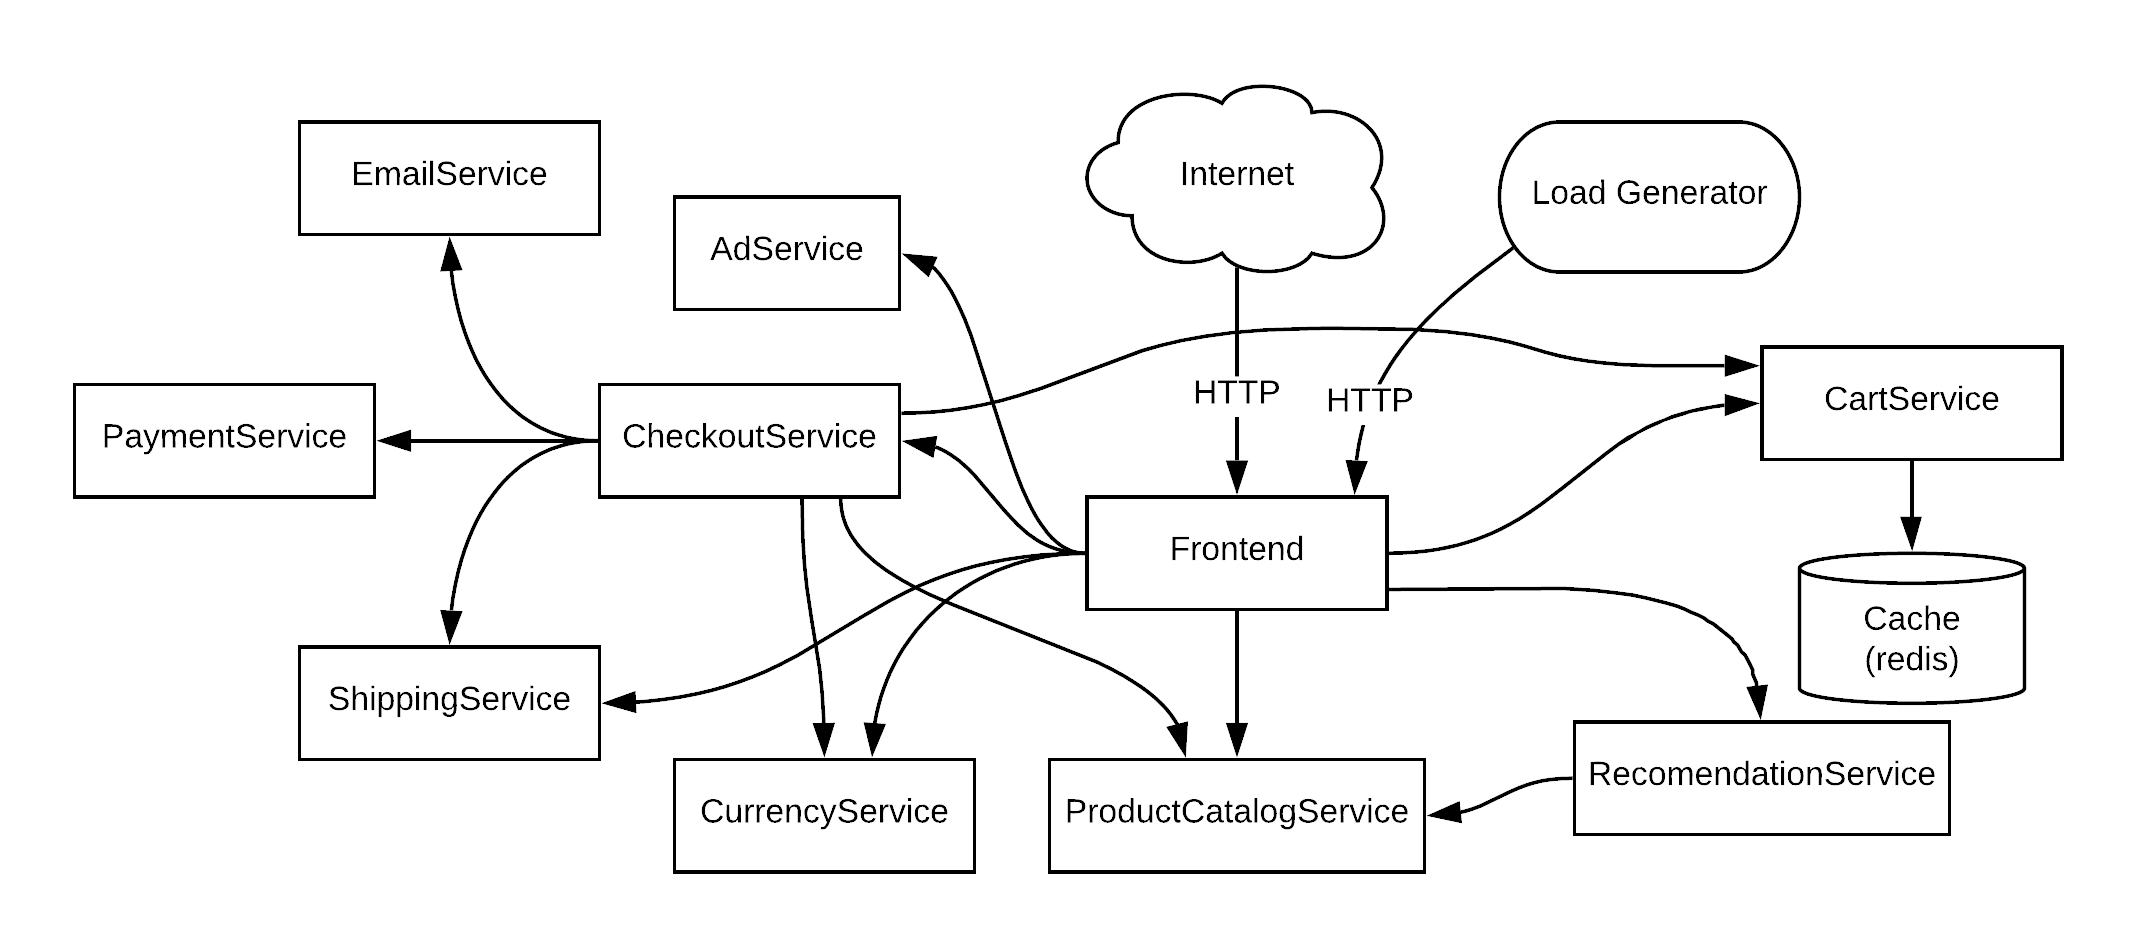
\includegraphics[width=1\textwidth]{resources/ch4/hipster-arch.png}
	\caption{Arsitektur aplikasi Hipster Shop}
	\label{butiq-arch}
\end{figure}

\subsection{Metode Pengujian}
Untuk melakukan pengujian pada sistem PRA yang telah dibuat, \textit{service} yang ada pada Hipster Shop akan dimodifikasi untuk meniru perilaku dari \textit{service} yang mengalami regresi kinerjan. Ada dua metode utama yang dapat dilakukan untuk membuat perilaku regresi pada \textit{service} yaitu dengan menambahkan perintah \textit{sleep} dan juga menambahkan kalkulasi matematika terutama perhitungan fungsi trigonometri yang membutuhkan banyak usaha dari CPU untuk menyelesaikannya sehingga diharapkan fungsi-fungsi tersebut akan memiliki \textit{latency} yang lebih besar. Tabel \ref{modified-function} menunjukkan fungsi-fungsi yang akan dimodifikasi pada \textit{service}-\textit{service} untuk meniru perilaku regresi.
\begin{small}
	\begin{longtable}{ | p{1cm} | p{5cm} | p{5cm} | }
		\caption{Daftar fungsi yang akan dimodifikasi}
		\label{modified-function}                                                           
		\\ \hline
		\centering\bfseries{No} & \centering\bfseries{Nama Service} & \centering\bfseries{Nama Fungsi} \tabularnewline \hline
		\endfirsthead
%		1 & AdService &  cookware \\ \hline
		1 & CheckoutService &  placeorder \\ \hline
		2 & CurrencyService &  convert \\ \hline
		3 & EmailService &  sendorderconfirmation \\ \hline
		4 & PaymentService &  charge \\ \hline
		5 & ProductCatalogService &  getproduct \\ \hline
		6 & RecommendationService &  listrecommendations \\ \hline
		7 & ShippingService &  getquote \\ \hline		
	\end{longtable}
\end{small}






\subsection{Hasil Pengujian}
Berikut adalah hasil pengujian yang telah dilakukan pada sistem PRA.
